{\Huge\textbf{ DELETE THIS PAGE}}
\section{Poznámky - informačný účel}
Táto strana slúži na poznámky, TODO, toho čo mám ešte urobiť. 
Bude samozrejme zmazaná.  
Dany text, ktory sa bude dat pouzit v praci bude presunuti do jadra prace. 

dopnit do praktickej casti mapu: vyuzivajuc tento priklad ovladania.. \url{http://raphaeljsvectorgraphics.com/the-graphical-web/turtle-graphics-logo}
pozriet si funkciu snap - inAnim()...

\newpage
\section{Learning Raphael JS Vector Graphics}
%V práci cituj: \cite{Dawber} , strany sa cituju takto: \cite[p.~215]{Dawber} \\ Priklady z knihy:\url{http://raphaeljsvectorgraphics.com/}  \cite{Dawber} .
%Z tejto knihy idem pridávať do bakalárky nasledovné veci:
%Namet na zmenu: pouzit to demo, ktore mi poslal veduci na transformaciu zmeny. 


\subsection{Porovnanie spôsobu vykreslenia cez SVG SMIL a Snap}

Kreslenie vektorov je jednoduchšie cez Snap ako čisto písanie SVG. 

Príklad kreslenia obdĺžníka a animovanie šírky z 50 pixlov na 100 pixelov cez čisté SVG:\cite[p.~9]{Dawber}
\begin{lstlisting}
<svg>
<rect x="10" y="10" width="50" height="30">
	<animate attributeType="XML"
		attributeName="width"
		to="100"
		fill="freeze"
		dur="10s"  />
</rect></svg>
\end{lstlisting}

Nakreslíme obdĺžnik na súradniciach (10, 10) s šírkou 50, a výškou 30 použitím elementu $<$rect$>$. Zoskupený element $<$animate$>$ definuje animáciu zmeny šírky obdĺžnika na šírku 100 px, ktorá trvá desať sekúnd. Kde fill="freeze" je použité na zachovanie stavu obdĺžnika po ukončení animácie. Inak by bola nastavená na 50. 

Ekvivalent k animácii cez Snap API v nasledujúcom príklade:

\begin{lstlisting}
paper = Snap();
var rect = paper.rect(10, 10, 50, 30);
rect.animate({
	width: 100
	}, 10000);
\end{lstlisting}

Syntax metód animate a rect je výstižnejšia a lepšia na pochopenie. Snap sa tiež dobre integruje s inými knižnicami, ako napríklad jQuery. 


%%%%%%%%%%%%%%%%%%%%%%%%%%%%%%%%%%%%%%%%%%%%%%%%%%%%%%%%%%%%%%%%%%%%%%%%%%%%%%%%%%%%%%%%%%%%%%%%%%%%%%%%%%%%%%%%%%%%%%%%%%%%%%%%%%%%%%%%%%%%%%%%%%%%%%%%%%%%%%%%%%%%%%%%%%%%%%%%%%%%%%%%%%%%%%%%%%%%%%%%%%%%%%%%%%
\newpage
%Jednoduche kreslenie ,
%Interakcia ,
%Animovanie.. 
%
%Krok 0: ziskanie Snapu...

 
\subsection{Krok 1: Inicializácia plátna na kreslenie}
%viewport = výrez
Na to, aby sme boli schopní kresliť grafické komponenty, tak potrebujeme definovať miesto, kde budú vykreslené. 
%Určenie miesta, kde bude vykreslené plátno je buď viditeľné okno vo webovom prehliadači, alebo viewport. 
Viditeľná oblasť okna prehliadača, alebo viewport, definuje oblasť, v ktorej sa vykreslí komponent na plátno.
SVG špecifikácia referuje ako miesto vykreslenia seba ako viewport. 
Inak povedané viewport je akákoľvek obdĺžniková oblasť.
Okno prehliadača je referencia na viewport a kresliaca oblasť je plátno.   \cite{Dawber}


Vytvorenie plátna cez Snap konštruktor sa dá urobiť viacerými spôsobmi.

\subsubsection{Súradnice plátna}
 
 
Nasledujúci príkaz zadefinuje pláno s rozmermi šírka je 300 a výška 200. 
\begin{lstlisting}
var paper = Snap(300, 200);
\end{lstlisting}


Na obrázku \ref{fig:suradnice1}  je znázornená východzí súradnicový systém plátna vytvoreného cez Snap konštruktor. 
Začiatok súradnic na osi x, y je rovné nule. Bod na plátne so súradnicami x = 300, y = 200 alebo (300, 200) vo vektorovom zápisu je bod 300px vpravo od začiatku x-ovej osi a 200px dole od počiatku y-ovej osi. 

\begin{center}
	\begin{figure}[hp]
\centering
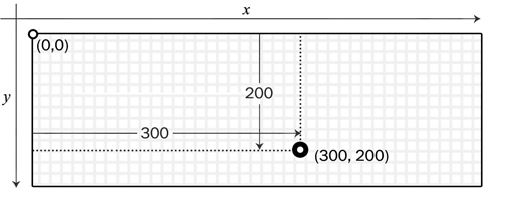
\includegraphics[width=0.7\linewidth]{obrazky/suradnice1}
\caption{Súradnicový systém plátna s bodom (300, 200)}
\label{fig:suradnice1}
\end{figure}
\end{center}


\subsubsection{DOM element}

Dosť často je potrebné použiť existujúci DOM element ako kontajner pre plátno než viewport. Ako element môžeme použiť napríklad:
\begin{lstlisting}
 <div id="mojePlatno"></div>  
 \end{lstlisting}

Nasledujúcim kódom vytvorím 500px široké a 300px vysoké plátno.

\begin{lstlisting}
var paper = Snap("mojePlatno", 500, 300);
\end{lstlisting}

Keď využívam túto formu konštruktora, tak prvý element je ID elementu. Alternatívne sa dá prvý parameter DOM element napísať nasledovným spôsobom: 
\begin{lstlisting}
Snap(document.getElementById('mojePlatno'), 500, 300);
\end{lstlisting}


\newpage

\subsection{Kreslenie základných tvarov cez Snap}


